\chapter{Design ESB in Openshift}
\label{cha:esboc}
In this chapter, the ESB integration example of Section \vref{sec:esb-integration-example} will be designed as microservices, which can run on a Openshift Cluster. An Openshift Project will act as the ESB, which will provide the mediation, security, configurations and secrets for the services. The concrete functionality of the services is considered to be not important. The goal is to redesign the service components of Figure \vref{fig:esb-design-sca} as microservices, and to design the Openshift Project, which will host the services, and act as the ESB. \\

As discussed in Chapter \vref{cha:esb}, an ESB is a distributed computing architecture, whereby services act as a consumer or producer. These services provide a business value for an enterprise in form of an integration of an internal or external service. There are multiple providers of ESB middleware like JBoss Fuse, which provide tooling for implementing service components running on the ESB middleware. The prototype will illustrate that SOA service components can be implemented as microservices, whereby features provided by the ESB middleware, such as bindings will have to be replaced by other implementations.

\section{Microservice Architecture}
Figure \vref{fig:esboc-design-services} illustrates the microservice architecture of the integration example of Figure \vref{fig:esb-design-sca}. Conceptually, the transformation of a service component to a microservice is easy, because a service component and a microservice act very similar. Compared to a service component of an ESB middleware, a microservice is completely separated from the other services, brings in its own libraries, and runs in its own runtime environment. From the implementation point of view, the microservices need to provide an runtime environment, which was previously provided by the ESB middleware. Therefore, that the microservices are completely separated, the access of other services is not mediated as usual anymore, because the communication is now performed via standard protocols like HTTP(S). In a monolithic ESB application, running on JBoss EAP, every service component is accessed via a reference, whereby the reference proxies the request directly to the service, which is running in the same runtime environment. With microservices, running in their own runtime environment, it is not possible to access the service instance directly anymore. Only communication via standard protocols, such as HTTP(S), is supported.

\begin{figure}[htbp]
	\centering
	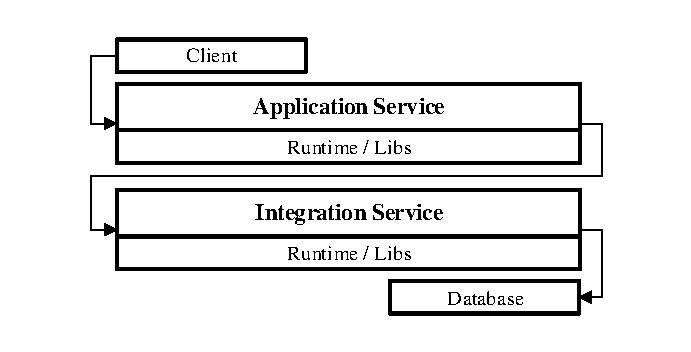
\includegraphics[scale=1]{images/esboc-design-microservice.pdf}
	\caption{Microservice architecture}
	\label{fig:esboc-design-services}
\end{figure}

\section{Microservice Aspects}
\label{sec:esboc-aspects}
This section will discuss the necessary aspects of microservices, which will ensure, that the services are properly implemented, and can effortlessly be managed. Especially the monitoring of the services becomes very important, when moving from a conventional monolithic ESB application, like an application running on JBoss Fuse, to a microservice architecture based ESB application. Services running as microservices on Openshift, are running in their own runtime environment, and therefore cannot share any runtime resources. \\

Figure \vref{fig:esboc-aspects} illustrates the hierarchy of the microservice aspects, which will ensure that the implemented services are
\begin{itemize}
	\item secure,
	\item configurable for multiple environments,
	\item observable by developers and operators,
	\item resilient to failures
	\item and measurable.
\end{itemize}

The prototype will be implemented in Java, whereby the Eclipse community has provided the MicroProfile specifications, which provide an API to cover most of the microservice aspects. Using the MicroProfile specifications decreases the implementation effort, and provides an standardized way to implement microservices\cite{EclipseMicroprofileCharter2017}. \\

The following sections will specify the microservice aspects for the to implement microservices. 

\begin{figure}[htbp]
	\centering
	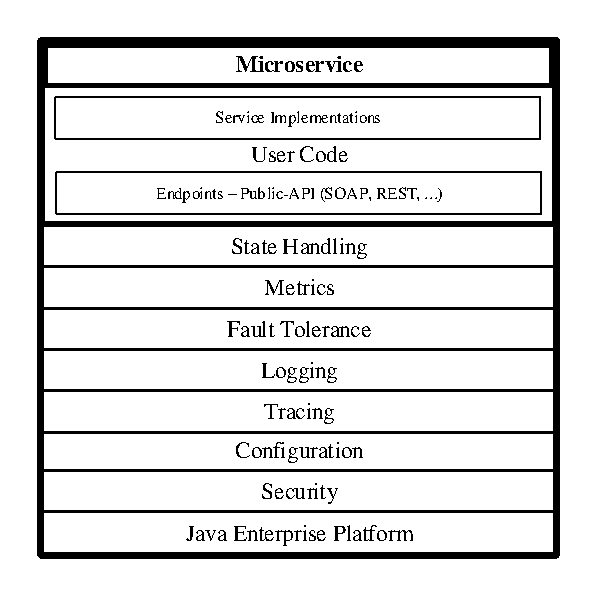
\includegraphics[scale=1]{images/esboc-requirement-services.pdf}
	\caption{Service Requirements}
	\label{fig:esboc-aspects}
\end{figure} 

\subsection{Security}
\label{sec:esboc-aspects-security}
Distributed services need to be secured properly from unauthorized access, therefore the microservices will be secured with OAuth2. OAuth2 is a token based authentication scheme, which has become popular over past few years. There are several open source implementations for interacting with an authentication service via the OAuth2 scheme. The Integration Service must authenticate its client, the Application Service, against an central authentication service, whereby the Application Service will retrieve the access tokens from the central authentication service, and the Integration Service validates the provided token against the central authentication service\cite{OAuth2018}.

\subsection{Configuration}
\label{sec:esboc-aspects-config}
The Eclipse MicroProfile specifications provide the MicroProfile-Config specification, which provides an API to inject configuration parameters into CDI Beans. The injected configuration parameters are loaded from so called configuration sources. A configuration source can either be Java System-Properties, Environment Variables, Properties Files, YAML Files or custom implementations, for instance, to retrieve configurations from a database. The services must be implemented in a way, to be configurable for different stages such as DEV (development) and PROD (production), whereby  the services are only allowed to use configuration parameters via injection\cite{EclipseMicroprofileConfig2018}.

\subsection{Tracing}
\label{sec:esboc-aspects-tracing}
The Eclipse MicroProfile specifications provide the MicroProfile-OpenTracing specification, which provides an API for tracing an application on a method level and across service boundaries. Distributed tracing allows to comprehend service or method call chains of distributed services. There is open source tooling available to analyze the collected tracing data, provided by the distributed services. The services must collect reasonable tracing information and send this data to a central tracing service\cite{CNCFOpentracing2018}.

\subsection{Logging}
\label{sec:esboc-aspects-logging}
Distributed logging allows to comprehend logs across service boundaries, within a service call chain, whereby the logs of all involved services have to be marked with the same transaction id. There is open source tooling available to analyze the collected logs, provided by the distributed services. The services must provide all of their logging to a central service, whereby the logs must be marked with a transaction id, which is provided by the MicroProfile-OpenTracing API. Optionally, the services are allowed to add additional markers, which can help developers and operators to analyze problems or to group service logs.

\subsection{Metrics}
\label{sec:esboc-aspects-metrics}
The Eclipse MicroProfile specifications provide the MicroProfile-Metric specification, which provides an API to define and manage metrics. Metrics allow to comprehend the state of a microservice, such as resource consumption, API calls or failure counts. Metrics along with distributed tracing and distributed logging, provide the necessary data, developers and operators need to analyze failures in services, which occurred in service call chains. The services must collect reasonable metrics and publish those metrics, which can be made available to a central metric service\cite{EclipseMicroprofileMetrics2018}.

\subsection{Fault Tolerance}
\label{sec:esboc-requirements-service-fault}
The Eclipse MicroProfile specifications provide the MicroProfile-FaultTolerance specification, which provides an API to define fault tolerance behavior such as retries, timeouts and error fall-backs. The fault tolerance of a service means, that if a depending service is not accessible at the time, a service must not fail immediately after the first try, but the service should retry to call the depending service for several times, and fail, when all retries have failed. Such a behavior ensures that short timed communication errors, redeployments or overloads do not immediately cause a service to fail. The services must provide proper fault tolerance configuration and fall-back behavior, to be able to recover from such errors in a proper manner\cite{EclipseMicroprofileFault2018}.   

\subsection{API Management}
\label{sec:esboc-requirements-service-api}
The API management of a public API such as REST API and REST Models ensure, that the clients, using the public API, are not broken by changes, made on that API. There are several opinions on how API management can be done. A public API has to be stable per design, and needs to evolve and provide backward compatibility in a way, so that clients have enough time to catch up with the changes. Swagger has become very popular for documenting an API, whereby the documentation can be used to generate clients, provide documentation for developers and to test the public API. The services must be capable of migrating their public API in a way, that the clients are not broken by made changes. The services must provide a Swagger Documentation, and provide a capability to access the Swagger Documentation\cite{SmartBearSwagger2018, RestVersion2018}.

\section{Openshift Architecture}
\label{sec:esboc-design-oc}
Figure \vref{fig:esboc-design-openshift-project} illustrates the design of the Openshift Project, which will act as the ESB. As discussed in Section \vref{sec:paas-openshift-project}, Openshift isolates Kubernetes Namespaces  by bringing in the concept of an Openshift Project. Services in an Openshift Project, which are not exposed via an Openshift Route, are implicitly protected from access from external networks, and other Openshift Projects. The Openshift Project will contain the Application Service, the Database Service and the Integration Service. The Application Service has access to the Internet, and will be accessed by the Client from the Internet via its public address. The Integration Service and the Database Service are not exposed to the Internet, and can only be accessed within the Openshift Project by their service names.

\begin{figure}[htbp]
	\centering
	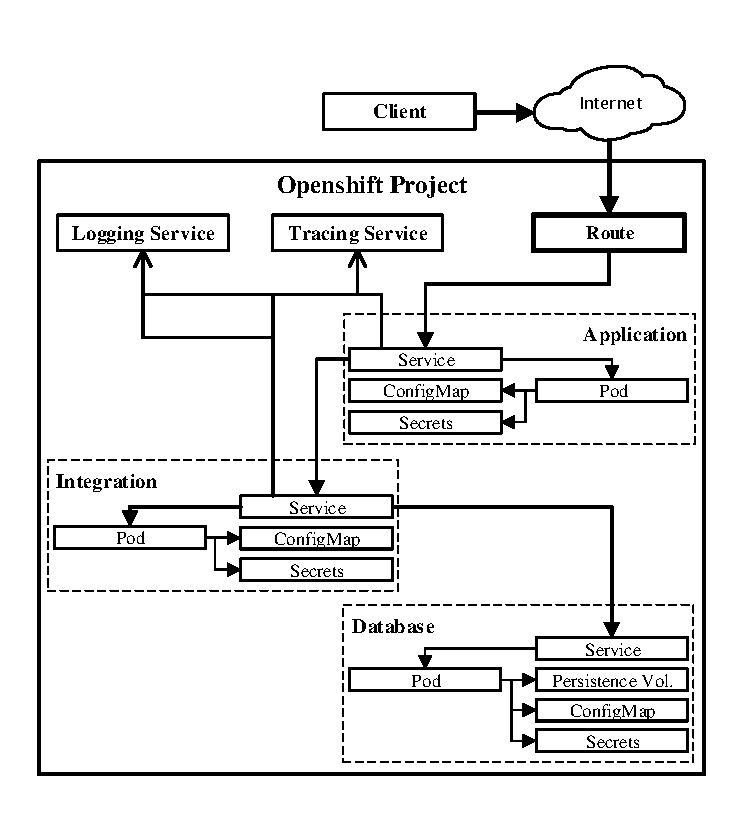
\includegraphics[scale=1]{images/esboc-design-openshift.pdf}
	\caption{Openshift Project architecture}
	\label{fig:esboc-design-openshift-project}
\end{figure} 

All services provide their tracing and logging data to external services, whereby no special configuration will be needed in Openshift, because Openshift allows services to access external resources. The mediation of the services is managed by Openshift Service objects, whereby the services communicate with each other via their service names, which ensures, that the communication stays within the Openshift Project. The Openshift Project must manage all configurations and secrets, which can be referenced by the services.

\section{Openshift Requirements}
\label{sec:esboc-requirements-oc}
The implementation of the Openshift Project such as templates and scripts, must be implemented under consideration of the principles of IaC, which have been discussed in Section \vref{sec:iac-principles}. Sticking to the principles of IaC will ensure, that the Openshift Project can effortlessly be managed and reproduced on any Openshift Cluster. \\

The Openshift Project will host the services and manage their configurations and secrets via Openshift ConfigMaps and Openshift Secrets, which have been discussed in Section \vref{sec:caas-kubernetes-objects}. The configurations and secrets are managed outside the service code bases, and are provided by the Openshift Project for a specific stage, the Openshift Project represents. The configurations and secrets are supposed to be managed by operators, and are only made available to the services during runtime, and shouldn't be accessible by developers. \\

The services must manage their integration into Openshift, by providing the necessary templates, whereby configurations and secrets are referenced by their predefined names and keys. The services must expose all necessary configuration parameters, which allow to configure the service for a specific stage, whereby the Openshift Project will provide the proper configuration and secret values for the specific stage. \\

For demonstration purpose, the Openshift Project, representing the ESB, will host a tracing service and a log aggregation service as well. This is due to the fact, that in shared environments, the customers have limited privileges, and therefore, not all configurations of Openshift are available. \\

The following chapter will discuss the implementation of the designed prototype. 
